\documentclass[norsk, twocolumn,letterpaper,11pt,fleqn]{extarticle}
\usepackage[norsk]{babel} 
\usepackage[utf8]{inputenc} 
\usepackage{times}			% Default times font style
\usepackage[T1]{fontenc} 	% Font encoding
\usepackage{amsmath} 		% Math package
\usepackage{mathtools} 		% Adds the declare paired 
							% delimeter command to make costom \abs and \norm
\usepackage{breqn}		 	% Adds dmath environment for automated brakeline
\usepackage{xfrac}			% Adds slanted fractions (sfrac)
\usepackage{cancel}			% Adds the cancel command, a slash through the symbol(s)
\usepackage{tabularx}		% Adds adjustable width on tabulars
\usepackage{cuted}			% Adds the strip command, pagewidth text in a twocolumn
							% environment.  
\usepackage{hyperref}
\usepackage[letterpaper, margin=0.6in]{geometry}
\usepackage{parskip}		% Norske avsnitt
\usepackage{siunitx}		% SI-enheter
\usepackage{tablefootnote}
\usepackage{tabularx}
\usepackage{listings}

% Alghorithm packages:
\usepackage{algorithm}
\usepackage[noend]{algpseudocode}

% Start custom \abs \norm 
\DeclarePairedDelimiter\abs{\lvert}{\rvert}%
\DeclarePairedDelimiter\norm{\lVert}{\rVert}%
% Swap the definition of \abs* and \norm*, so that \abs
% and \norm resizes the size of the brackets, and the 
% starred version does not.
\makeatletter
\let\oldabs\abs
\def\abs{\@ifstar{\oldabs}{\oldabs*}}
%
\let\oldnorm\norm
\def\norm{\@ifstar{\oldnorm}{\oldnorm*}}
\renewcommand{\ALG@name}{Algoritme}
\makeatother
% End custom \abs \norm 

\usepackage{titlesec}
\titleformat{\section}[block]{\bfseries\filcenter}{\thesection}{1em}{\uppercase}
\titleformat{\subsection}[hang]{\bfseries\filcenter}{\thesubsection}{1em}{}
\titleformat{\subsubsection}[hang]{\bfseries\filcenter}{\thesubsubsection}{1em}{}

% TODO: Put comments on this section.
\newcommand{\eq}[1]{{\small\begin{align*}#1\end{align*}}}
\newcommand{\equ}[1]{{\small\begin{align}#1\end{align}}}
\newcommand{\mat}[1]{\begin{matrix}#1\end{matrix}}
\renewcommand\vec[1]{\mathbf{#1}}
\newcommand{\OP}[1]{\mathbf{\widehat{#1}}}
\newcommand{\op}[1]{\hat{#1}}
\newcommand{\unit}[1]{\mathbf{\hat{#1}}}
\renewcommand{\thesection}{\Roman{section}.}
\renewcommand{\thesubsection}{\Alph{subsection}.}
\renewcommand{\thesubsubsection}{\arabic{subsubsection}.}

\title{}

\begin{document}

\twocolumn[{%
 \centering
 {\small\MakeUppercase{Prosjektoppgave i FYS2130}}\\
 {\bfseries\large Måling og analysering av lyd}
 \\[1em]
 \normalsize \textit{Kandidatnummer:} 135
 \\
 	\begin{abstract}
		Denne rapporten er todelt. Den studerer hvordan man kan sette opp en audiometritest
		og lage audiogrammer for å analysere hørsel og hørselsvekking,
		samt lage en decibelmåler for å analysere støyende omgivelser.
		I rapporten viser jeg hvordan man kan programmere både et audiometer
		og en decibelmåler, basert på matematiske modeller og fysikk. 
		Resultatet er to praktisk anvendelige verktøy som blir brukt for
		å vise sammenheng mellom alder og hørselsvekking, og som viser at det er
		mye potensielt skadelig støy i bybildet og inne i bygninger.
		Rapporten konkluderer med at det er mange utfordringer knyttet til 
		både audiometri og støymåling, og at det er særdeles viktig å kunne 
		kalibrere verktøyene mot profesjonelt utstyr.
 	\end{abstract}
 \\[3em] % some more space after the title part
}]

\section{Introduksjon}
\label{sec:intro}
\subsection{Audiometri og lyd}
\label{sub:audio}
Lydenergi beveger seg i bølger, 
og som for andre bølger, er formen bestemt av bølgens \textit{amplitude} $A$ 
og \textit{frekvens} $f$.

Amplituden er et mål på bølgens \textit{intensitet}, og kommer av at bølgen lager et 
\textit{lydtrykk} $p$ i luften, angitt i enhet [\SI{}{\W\per\meter\squared}]. 
Forholdet mellom intensitet og trykk er
\equ{
	I = p^2
}

Lydintensiteten påvirker ikke øret vårt lineært, 
så å måle lydtrykket i arbeid per kvadratmeter, er ofte lite ønskelig.
Vi bruker derfor heller en logaritmisk \textit{decibelskala}, 
som måler lydtrykket opp mot en referanseverdi. Decibelskalaen \textit{SPL} 
(\textit{sound pressure level}) har formen
\equ{
	L = [10\;\text{db(SPL)}]\log \frac{I}{I_{ref}}
	= [10\;\text{db(SPL)}]\log \frac{p^2}{p^2_{ref}}
\label{eq:Iref}}
der $I_{ref} \sim$ \num{e-12} \SI{}{\W\per\meter\squared}, og er definert ut ifra lyd med
frekvens \num{1000} \SI{}{\Hz}, 
og lydtrykk $p_{rms} = 20$ \SI{}{\micro\Pa} («root mean square»-verdi). 
Dette er en ofte brukt absolutt dB-skala. I dette prosjektet  
skal vi bruke \textit{dB(A)-skalaen} (seksjon \ref{sec:met} \ref{sub:dba}).

Lydens frekvens måles i antall svingninger per sekund. 
Menneskeøret er et sensitivt organ, og kan oppfatte lydbølger med
frekvenser mellom \num{20} og \num{20 000} \SI{}{\Hz}, 
men det skiller best frekvenser mellom 
\num{2 000} og \num{5000} \SI{}{\Hz}. Det betyr at når man måler lyd, vil man gjerne
ta hensyn til dette, og derfor vekte målingene deretter.

For å teste hørsel, brukes et \textit{audiometer}. 
Audiometeret spiller av korte toner
med forskjellige frekvenser for en forsøksperson, og målet er å kartlegge ved hvilke
lydintensiter forsøkspersonen ikke lenger hører de forskjellige frekvensene.
Deretter presenteres dataene fra forsøket i \textit{audiogram}, ett for hvert øre,
og sammenlignes med hørselen til en «normalperson», 
representert ved en 
\textit{minimum audibility curve}\footnote{I. Khurana, 
Medical Physiology for Undergraduate Students, 2014, s. 931}
for forskjellige frekvenser. Den laveste lydintensiteten et fullfungerende menneskeøre
kan høre, er gitt ved \num{0}-phon-kurven. \num{0} phon er definert
ved $I_{ref}$ i likning (\ref{eq:Iref}).

I slike tester brukes som oftest hodetelefoner som dekker hele øret.
Utfordringen ved dette, er at \num{0}-phon-kurven er definert fra tester der det brukes
høytalere, plassert en bestemt avstand fra forsøkspersonen, i et lydtett rom.
Vi nøyer oss derfor med å sammenligne absolutte forskjeller mellom forsøkspersonene.

Over tid kan man sammenligne resultatene for samme person, siden
hørselen svekkes med alderen, samt påvirkning fra intens lyd over tid 
(se tabell \ref{tab:tab1}).

\begin{table}[h!]
	\begin{tabular}{l|l}
		\hline
		Gjennomsnittlig lydintensitet & Tolerabel eksponeringstid\\
		\hline\hline
		85 \SI{}{\dB}(A) – travel bytrafikk & 8 timer \\
		\hline
		88 \SI{}{\dB}(A) & 4 timer \\
		\hline
		91 \SI{}{\dB}(A) & 2 timer \\
		\hline
		94 \SI{}{\dB}(A) & 1 time \\
		\hline
		97 \SI{}{\dB}(A) & 30 minutter \\
		\hline
		100 \SI{}{\dB}(A) & 15 minutter \\
		\hline
	\end{tabular}
			\caption[]{For hver 3 \SI{}{\dB} økning i intensitet, halveres anbefalt eksponeringstid\footnotemark[2].}							
	\label{tab:tab1}
\end{table}
\footnotetext[2]{http://www.cdc.gov/niosh/hhe/reports/pdfs/2002-0131-2898.pdf}			
\subsection{Lydmåling} 
\label{sub:lydmål}
I andre del av dette prosjektet ser vi på hvordan vi kan konstruere en lydmåler
ved hjelp av en mikrofon og et dataprogram. En slik lydmåler kan brukes til 
å undersøke støynivået i forskjellige situasjoner. I samfunnet i dag er det
en nødvendighet å kartlegge støynivået ved for eksempel sterkt trafikkerte veier,
jernbanelinjer eller byggeplasser, 
for å unngå at arbeidere skader hørselen ved lengre eksponering for høy lyd 
(se tabell \ref{tab:tab1}).

Utfordringene ved å lage en lydmåler er mange. Det er vitkig å få til en god vekting av
de ulike frekvensene, slik at resultatene samsvarer med profesjonellt utstyr. 
dB(A)-skalaen som vi skal jobbe med er mindre egnet for å ta opp lyd med høy intensitet,
men fordi det er den ledende standarden innen lydmåling, 
velger vi å prøve å optimalisere måleren for denne skalaen.

Et annet spørsmål man må ta hensyn til, er hvordan lyden skal tas opp.
Vi velger her å gjøre det ved å midle intensiteten over noen få sekunder,
og deretter se på intensiteten i både en relativ, uvektet dB-skala, 
og en relatic, dB(A)-vektet skala.

Når man har fått målt lyden, er det fortsatt en stor utfordring som gjenstår.
Hvordan velger vi referansepunktet slik at målingene våre gir mening?
Dette diskuteres videre i \ref{sec:met} \ref{sub:lydtest}.

\section{Metoder}
\label{sec:met}
\subsection{Oppsett av audiometer}
\label{sub:audiometer}
Som nevnt i seksjon \ref{sec:intro} \ref{sub:audio}, består første del av dette prosjektet
i å lage et fungerende audiometer som skal produsere audiogrammer for høyre og venstre øre
til en gruppe forsøkspersoner. 

Vi konstruerer en ren, tidsavhengig tone med en frekvens $f$ og amplitude $A$ på følgende måte
\equ{
	y = A\sin(2 \pi f t).}

Hvis man spiller av denne tonen uten noen modifiseringer, kan man risikere å høre en slags
«klikkelyd». Dette er veldig ugunstig når man tester toner med lave intensiteter.
Ved å øke amplituden gradvis ved inntoning, og tilsvarende reduksjon ved uttoning,
unngår vi denne «klikkingen». Dette gjøres ved å multiplisere tonen 
med en omhyllingskurve, og i denne rapporten bruker vi en 
\textit{sigmoid} funksjon (se figur \ref{fig:1} og \ref{fig:2}).

\begin{figure}[h!]
	\centering
	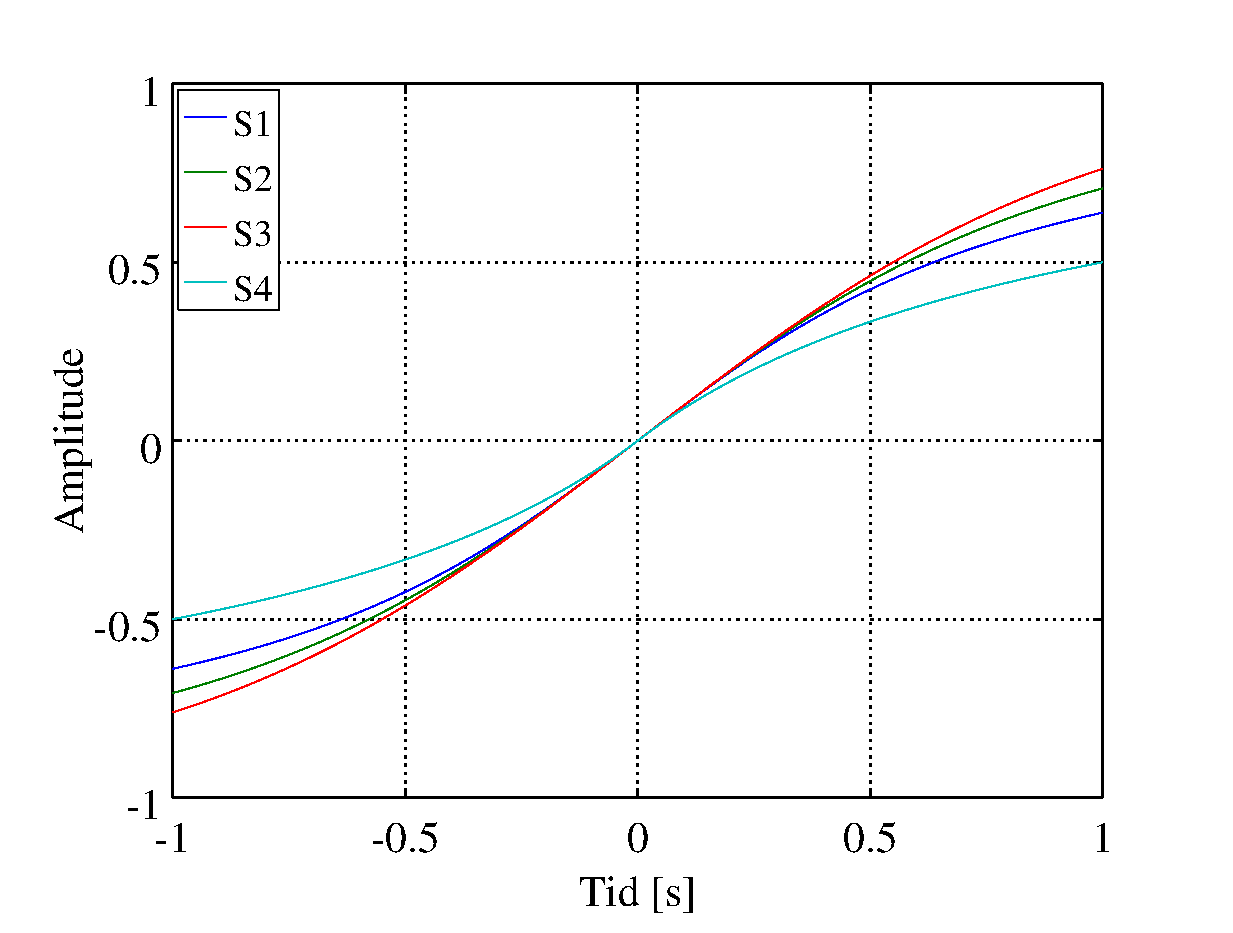
\includegraphics[width=100mm]{sigmoidsammenligning.eps}
	\caption[]{Fire sigmoide funksjoner.\\$S_1=(2/\pi)\arctan(\pi t/2)$, $S_2=t/(1+t^2)$\\ 
		$S_3=\tanh(t)$, $S_4=t/(1+|t|)$}
	\label{fig:1}
\end{figure}
\begin{figure}[h!]
	\centering
	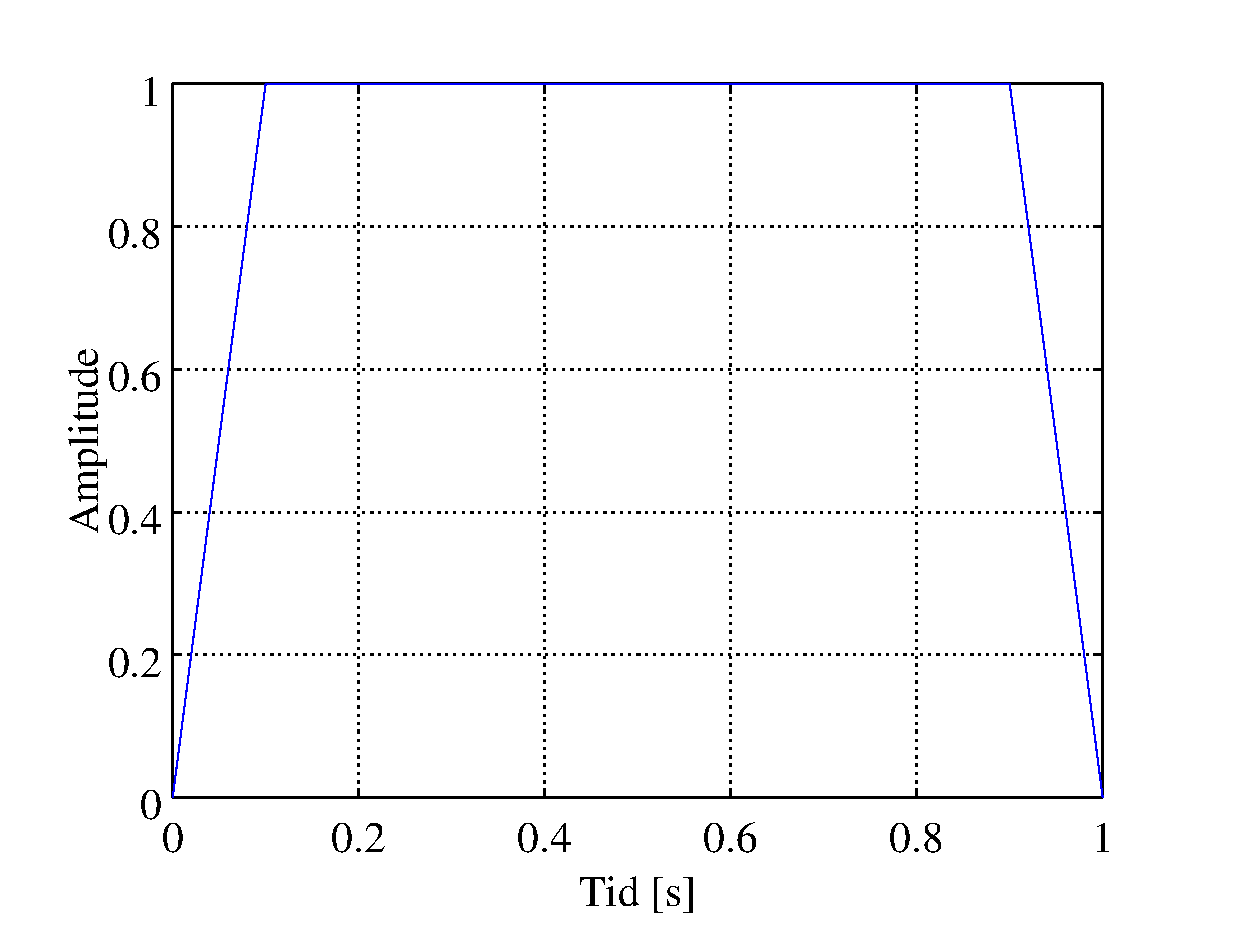
\includegraphics[width=100mm]{omhyll.eps}
	\caption[]{Omhyllingskurve gitt funksjonen $S_2$ multiplisert med en konstant.}
	\label{fig:2}
\end{figure}

I audiometeret vårt bruker vi $S_2$ multiplisert med en konstant, 
slik at den har verdi $1$ i $t=0{,}1$ s, og vi får en fin inn- og uttoning.

Programmet som kjører audiometridelen heter \textit{audiometri.m}, og
er relativt enkelt å bruke. Når man kjører programmet dukker det opp en prompt som
spør om du vil teste for høyre eller venstre øre, og deretter om du vil plotte
resultatet når testen er ferdig. Grafen lagres så til fil.

Selve testen utføres ved at brukeren utsettes for en lyd med én frekvens,
og lyden varer i ett sekund. Hvis brukeren ikke hører lyden, kan den justere opp
intensiteten med enten \num{1} eller \num{6} \SI{}{\dB} om gangen.
Hvis lyden er høy,
kan man justere ned intensiteten med \num{1} \SI{}{\dB}.
Når man har funnet den laveste intensiteten man kan høre, 
går turen videre til neste frekvens. Frekvensene som måles i dette forsøket er
[\num{60}, \num{120}, \num{250}, \num{500}, 
\num{1000}, \num{2000}, \num{4000}, \num{8000}] \SI{}{\Hz}.

Programmeringsdelen i dette prosjektet er gjort i \textit{Octave/Matlab},
og programlistingen er i vedlegg \ref{sub:ved1}

\subsection{Uvektet og vektet decibelskala}
\label{sub:dba}
For å kunne bruke en lydmåletest til noe nyttig, 
må vi ha en måte å sammenligne resultatene våre på.
Det gjør vi ved å finne frekvensspekteret ved hjelp av den fouriertransformerte 
av lydvektoren $y$,
og deretter regne ut en relativ intensitet ved å summere absoluttkvadratene av
frekvensspekteret. Til slutt normerer vi resultatet med hensyn 
på antall punkter i lydsamplevektoren.

Menneskeøret er som kjent ikke like 
sensitivt\footnote[3]{http://hyperphysics.phy-astr.gsu.edu/hbase/sound/earsens.html} 
for lyder ved alle frekvenser.
Vi bruker derfor også en 
\textit{A-vekting}\footnote[4]{http://en.wikipedia.org/wiki/A-weighting} for å
tilpasse programmet vårt til den mye brukte db(A)-skalaen.

Vektfunksjonen kan tilnærmes matematisk for en gitt frekvens $f$ på følgende måte
\eq{
	R_A(f) = \frac{12200^2\cdot f^4 \cdot (f^2+12200^2)^{-1}}
	{(f^2 +20{,}6^2)\sqrt{(f^2+107{,}7^2)(f^2+737{,}9^2)}}
}

En kan deretter regne ut relativ lydintensitet med db(A)-vekting slik
\equ{
	L_{dB(A)} = [10\;\text{dB(A)}]\cdot \log_{10} I_{dB(A)} + 2.0 - \text{dB}_{ref}
}
der vi finner den relative totale intensiteten ved
\equ{
	I_{dB(A)} = \frac{1}{N}\sum_{i=1}^N R_A(f_i)\cdot |g(i)|^2
}
der $g = \text{fft}(y)/N$ er «fast fouriertransformasjonen» av lyden vår.

\begin{figure}[h!]
	\centering
	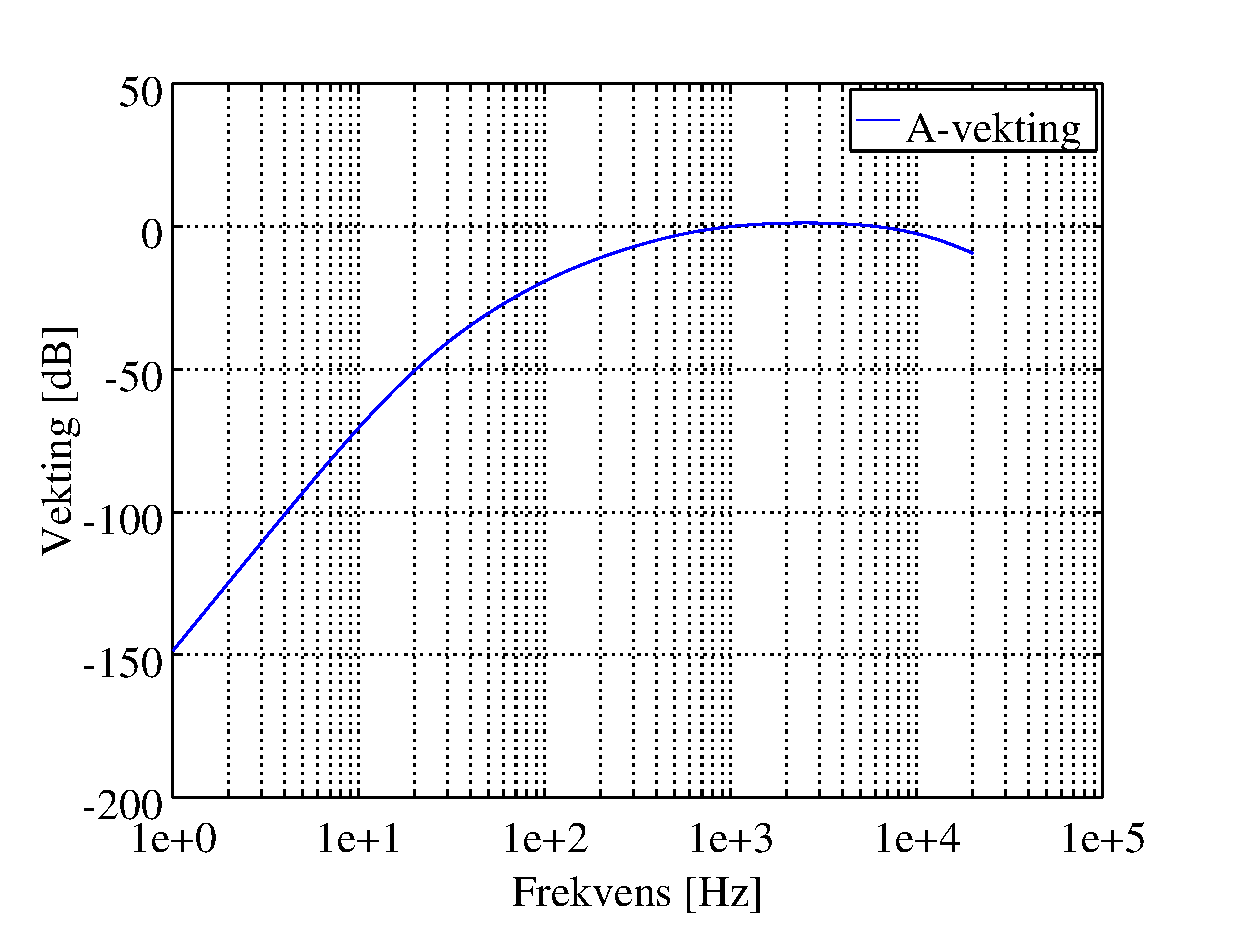
\includegraphics[width=100mm]{A-vekting.eps}
	\caption[]{A-vekting med funksjonen $20 \log_{10}R_A(f) + 2.0$. 
		Samsvarer med A-kurven\footnotemark[4]$^{,}$\footnotemark[5].}
	\label{fig:3}
\end{figure}\footnotetext[5]{A. I. Vistnes, Svingninger og bølger, 2015, s. 191}

\subsection{Lydmåling og -analyse}
Algoritme \ref{algo1} beskriver kort hvordan programmet \textit{measureSound.m} virker.
På grunn av speiling velger vi vekk halvparten av spekteret, og samtidig fjerner
vi det første elementet. Det er når «$f=0$», 
og der ligger gjennomsnittsverdien i spekteret,
som vi ikke trenger.
\label{sub:lydanalyse}
\begin{algorithm}[H]
	\caption{Lydopptak og fouriertransformasjon}\label{algo1}
  \begin{algorithmic}[1]
    \State{Sett Fs = \num{44 100}} \SI{}{\Hz}
    \State{Sett T $= 3$} \SI{}{\s}
    \State{Sett $N = 2^{17}$}
    \State{Sett ch = \num{2}}
    \State{Sett $M = N/2$}
    \State{Sett $f = 1{:}M$}
    \State $y=$ recordSound(Fs, T, ch)
    \State{$g = \text{fft}(y)/N$}
    \State{Initialiser vektorer $F$ og $F_A$}
    \For{For $i = 2,...,M$} 
    \State{$F(i) = |g(i)|^2$}
    \State{$F_A(i) = F(i)\cdot R_A(f_i)$}
    \EndFor
    \State{$I_{iv} =$ sum$(F(2{:}M))/N$}
    \State{$I_{A} =$ sum$(F_A(2{:}M))/N$}
    \State{dB$_{iv} =10\log_{10}I_{iv}- \text{db}_{ref}$}
    \State{dB$_A =10\log_{10}I_A + 2{,}0 - \text{db}_{ref}$}
  \end{algorithmic}
\end{algorithm}

Hovedprogrammene er her \textit{audiometer.m} og \textit{measureSound.m},
som bruker de andre, større funksjonene på en oversiktlig måte.
Filnavnene skal greit forklare hva funksjonen gjør, og funksjonene
er av forskjellig størrelse, avhengig av hva de skal gjøre.

\section{Tester}
\label{sec:testing}
\subsection{Audiometertesting}
Audiometeret ble testet på tre (fire med meg selv) forskjellige forsøkspersoner. 
Aldrene på de involverte var [18, 22, 24, 35] år, 
og det var to kvinner og to menn.
Alder og kjønn er også presentert i resultatdelen (står skrevet i figurbeskrivelsen).

Testen ble utført med øretelefoner som 
dekker hele øret\footnote[6]{http://www.razerzone.com/gaming-audio/razer-electra},
i et stille rom uten andre mennesker. Forsøkspersonene fikk prøve programmet
et par ganger før vi kjørte gjennom hele testen, og det er disse resultatene som
presenteres i neste seksjon.

Jeg valgte å bruke min egen hørsel ved \num{1000} \SI{}{\Hz} som referanseverdi,
siden jeg er relativt ung og har grei nok hørsel til at jeg burde ligge rundt normalen.

\subsection{Lydmålingstest}
\label{sub:lydtest}
Jeg kalibrerte lydmåleverktøyet i et delvis lyddempet rom, og jeg brukte en mobilapp
kalt «Sound Meter»\footnote[7]{Fra \textit{Smart Tools co.}} til å hjelpe meg.

Testingen av lydmåleren ble gjort i fire sammenhenger, 
og målingene er tidsmidlet over tre sekunder.

Den første målingen ble gjort på et kontor på Blindern på kveldstid, 
etter byggets stengetid. Den andre ble gjort inntil et litt støyende ventilasjonsanlegg.
Den tredje målingen ble tatt ut fra vinduet i en blokk, pekende mot ringveien.
Den fjerde målingen ble gjort i en park på kveldstid.
Noen av de mer konsistente verdiene som ble målt på de ulike 
stedene er tabulert i \ref{tab:tab2}.

En femte test for å se om det er samsvar mellom de vektede og uvektede decibelmålene,
er å teste for en tone på $1000$ Hz, siden det er den frekvensen dB(A)-skalaen
får størst utslag for. Ved å spille av en slik tone foran mikrofonen, fikk
jeg mange målinger der differansen mellom relativ dB og relativ dB(A),
var konsistent mellom $1$ og $2$, og målingene var jevnt over på samme nivå ($\sim 40$ dB).
Se tabell \ref{tab:tab2}.

\section{Resultater}
\label{sec:res}
\subsection{Resultater fra audiometri}
\label{sub:resaud}
Figurene $4$ til $11$ (se \ref{sub:vedb} for figurene 6 til 11) viser audiogrammer for 
ulike aldersgrupper og kjønn.
Selv om det er et i overkant snevert utvalg, 
er det interessant å se at resultatene stemmer godt overens med det vi vet fra teorien:
menn får dårligere hørsel tidligere enn kvinner, og unge under tretti år
har gjerne relativt god hørsel.

Det kunne vært enda mer interessant og sett audiogrammene hvis man hadde gjort testene
med høytalere i stedet for øretelefoner.
\begin{figure}[h!]
	\centering
	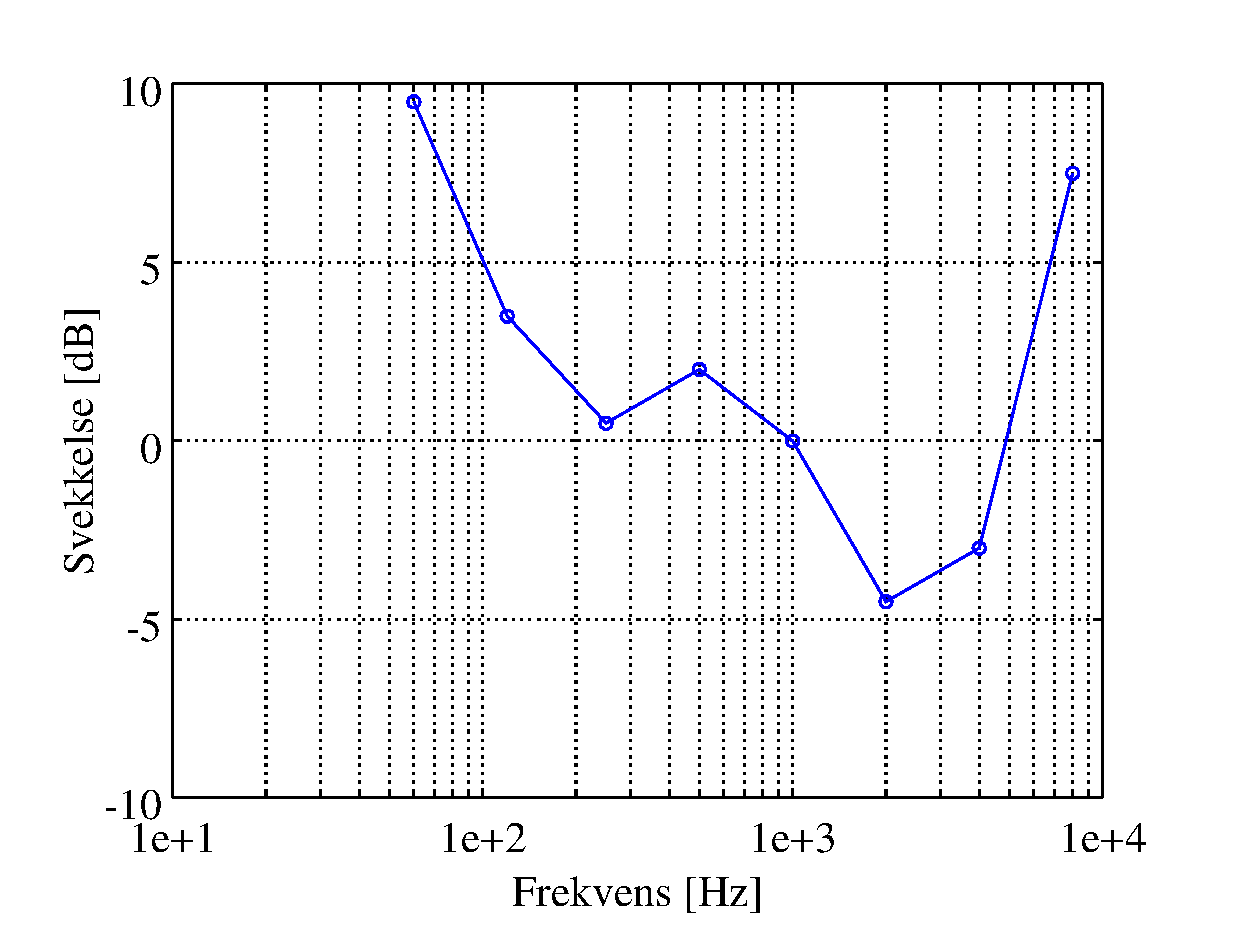
\includegraphics[width=100mm]{rightear.eps}
	\caption[]{Audiogram for 24 år gammel mann. Høyre øre.}
	\label{fig:4}
\end{figure}
\begin{figure}[h!]
	\centering
	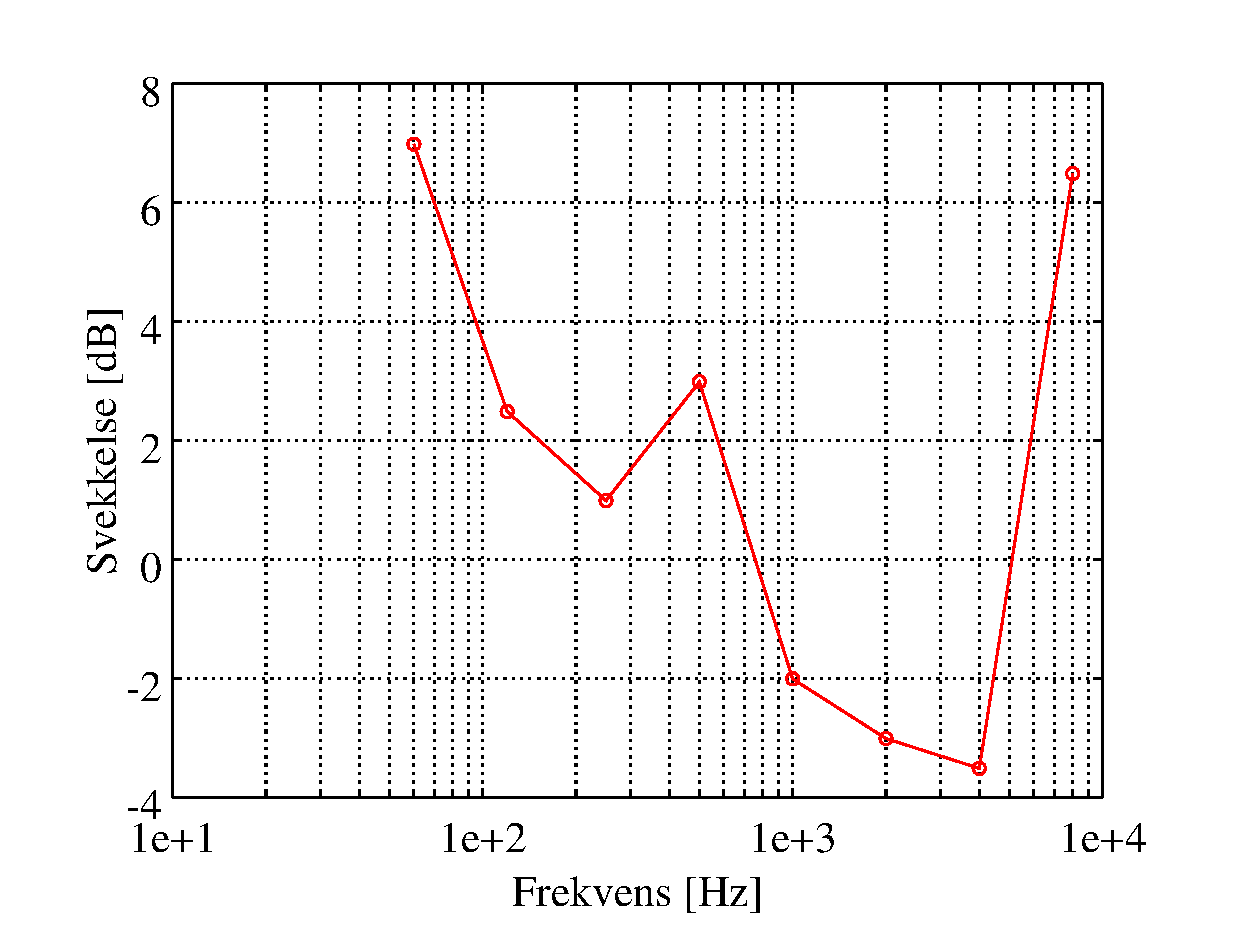
\includegraphics[width=100mm]{leftear.eps}
	\caption[]{Audiogram for 24 år gammel mann. Venstre øre.}
	\label{fig:5}
\end{figure}

\subsection{Resultater fra lydmålinger}
\label{sub:reslyd}
I tabell \ref{tab:tab2} ser vi resultatet fra decibelmålinger diverse steder
på og rundt Blindern.

Hvis vi ser på resultatene fra testen med den rene $1$ kHz-tonen,
ser vi at det er overraskende godt samsvar mellom vektet og uvektet dB-skala.
Både det at differansen mellom målingene er små, og det at målingene holder seg
jevnt på samme nivå, kan vise at lydmåleren gir gode resultater.

Siden vi jobber med relative lydintensiteter, er det veldig viktig at
lydmåleren gir konsekvente målinger. Selv om den ikke nødvendigvis er
kalibrert helt perfekt kan man i hvert fall måle forhold, 
samt måle forandringer i lydintensitet over tid, som man kan stole på.
\begin{table}[H]
	\begin{tabular}{l|l|l}
		\hline
		& dB$_A$ & dB$_{iv}$\\
		\hline\hline
		 Kontor & 30,9 & 33,1 \\
		\hline
		 & 31,3 & 34,0\\
		\hline
		 & 31,2 & 32,8 \\
		\hline\hline
		Ventilasjon & 66,6 & 76,7\\
		\hline
		& 64,8 & 76,7 \\
		\hline
		& 51,7 & 76,6 \\
		\hline\hline
		Mot vei & 59,0 & 75,4\\
		\hline
		& 63,3 & 76,0 \\
		\hline
		& 64,3 & 76,5 \\
		\hline\hline
		Park & 29,3 & 31,4\\
		\hline
		& 31,4 & 33,2 \\
		\hline
		& 30,5 & 32,6\\
		\hline
		$1000$ Hz tone & 40,6 & 41,7\\
		\hline
		& 40,9 & 42,1 \\
		\hline
		& 41,2 & 42,4 
	\end{tabular}
	\caption[]{Relative intensiteter i decibel, A-vektet og uvektet. Basert på tresekunders lydopptak.}							
	\label{tab:tab2}
\end{table}

\section{Konklusjon}
\label{sec:disk}
I denne rapporten har jeg prøvd å programmere en totalløsning
som er enkel å forstå, samt lett å bruke for noen som ikke nødvendigvis
kan programmering.

Vi har sett at resultatene fra både audiometeret og lydmåleren stemmer greit overens
med det vi forventet, selv om kalibreringen i lydmåleren sannsynligvis kan
jobbes mer med. Referansen til audiometeret er tatt ut fra mine testresultater,
så der er det også sannsynligvis forbedringspotensiale. Ved å teste i
lydtette rom, kan man også knytte resultatene opp til minimum audibility curve,
og få en bedre referanse til profesjonelle resultater på den måten også.

Gjennom å jobbe med denne rapporten ser jeg at det er flere store utfordringer
knyttet opp til lydmåling og audiometri.

\onecolumn
\appendix
\renewcommand{\thesubsection}{Vedlegg \Alph{subsection}:}
\renewcommand{\thesubsubsection}{\arabic{subsubsection}.}
\subsection{Programliste}
\label{sub:veda}
\rule{5cm}{0.1px}\\
{\bf audiometer.m:}

\lstinputlisting[language=Matlab]{../src/audiometer.m}
\rule{5cm}{0.1px}

\rule{5cm}{0.1px}\\
{\bf measureSound.m:}

\lstinputlisting[language=Matlab]{../src/measureSound.m}
\rule{5cm}{0.1px}

\rule{5cm}{0.1px}\\
{\bf recordSound.m:}

\lstinputlisting[language=Matlab]{../src/recordSound.m}
\rule{5cm}{0.1px}

\rule{5cm}{0.1px}\\
{\bf analyzeSound.m:}

\lstinputlisting[language=Matlab]{../src/analyzeSound.m}
\rule{5cm}{0.1px}

\rule{5cm}{0.1px}\\
{\bf playSound.m:}

\lstinputlisting[language=Matlab]{../src/playSound.m}
\rule{5cm}{0.1px}

\rule{5cm}{0.1px}\\
{\bf createSigmoid.m:}

\lstinputlisting[language=Matlab]{../src/createSigmoid.m}
\rule{5cm}{0.1px}

\rule{5cm}{0.1px}\\
{\bf sigmoid.m:}

\lstinputlisting[language=Matlab]{../src/sigmoid.m}
\rule{5cm}{0.1px}

\rule{5cm}{0.1px}\\
{\bf Ra.m:}

\lstinputlisting[language=Matlab]{../src/Ra.m}
\rule{5cm}{0.1px}

\rule{5cm}{0.1px}\\
{\bf dbaplot.m:}

\lstinputlisting[language=Matlab]{../src/dbaplot.m}
\rule{5cm}{0.1px}

\rule{5cm}{0.1px}\\
{\bf compareSigmoids.m:}

\lstinputlisting[language=Matlab]{../src/compareSigmoids.m}
\rule{5cm}{0.1px}
\newpage
\subsection{Flere figurer}
\label{sub:vedb}
\begin{figure}[h!]
	\centering
	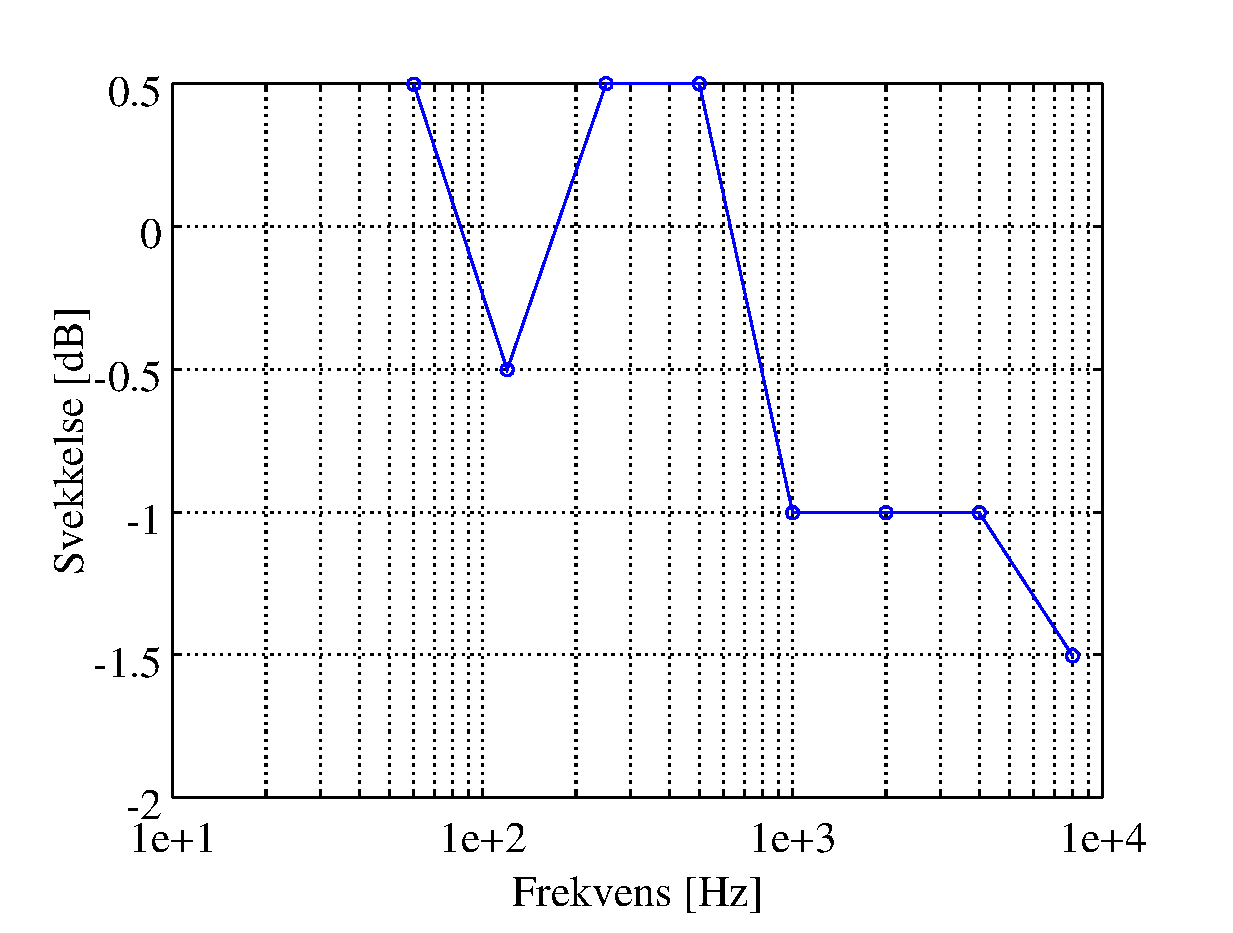
\includegraphics[width=100mm]{rightear22.eps}
	\caption[]{Audiogram for 22 år gammel kvinne. Høyre øre.}
	\label{fig:6}
\end{figure}
\begin{figure}[h!]
	\centering
	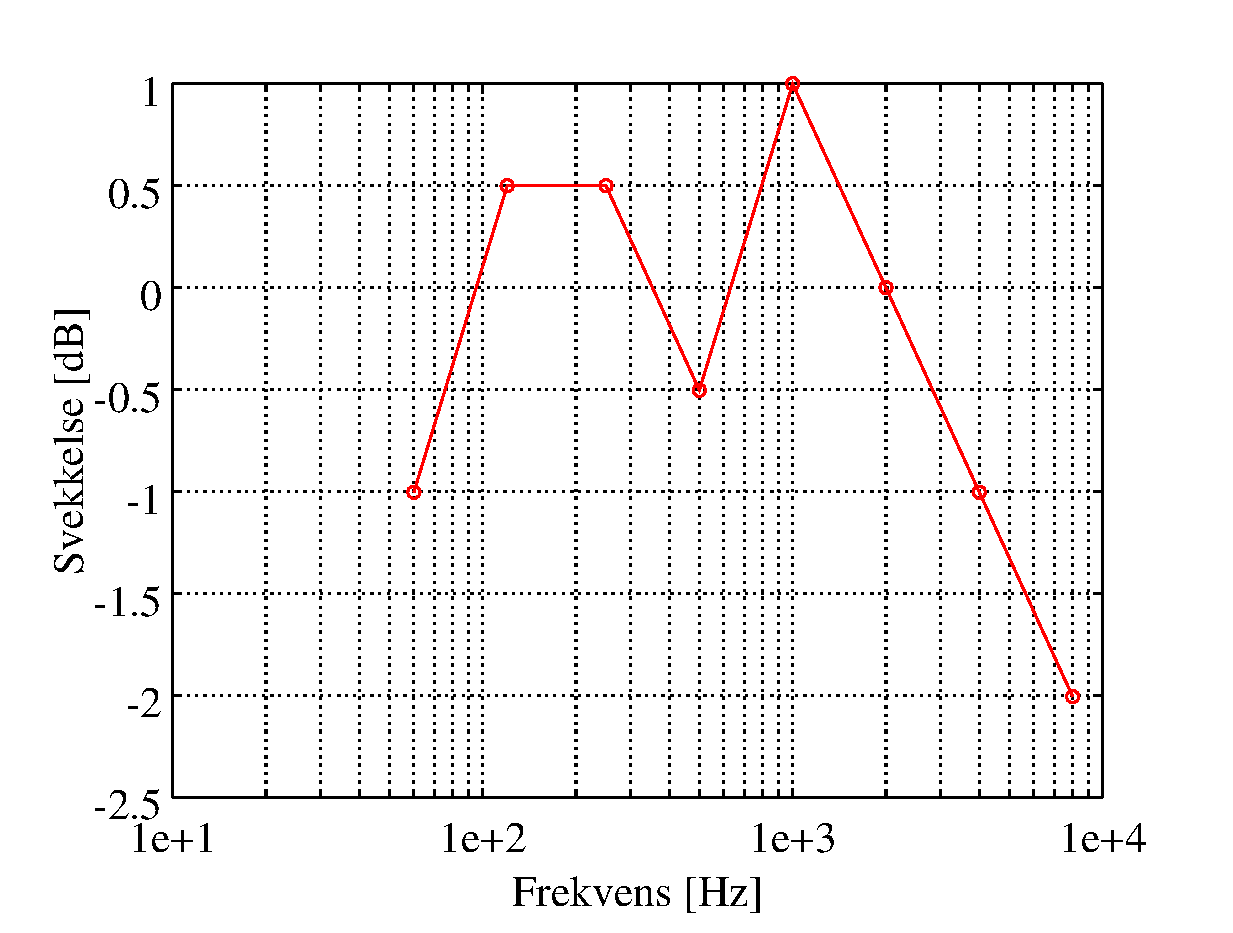
\includegraphics[width=100mm]{leftear22.eps}
	\caption[]{Audiogram for 22 år gammel kvinne. Venstre øre.}
	\label{fig:7}
\end{figure}
\begin{figure}[h!]
	\centering
	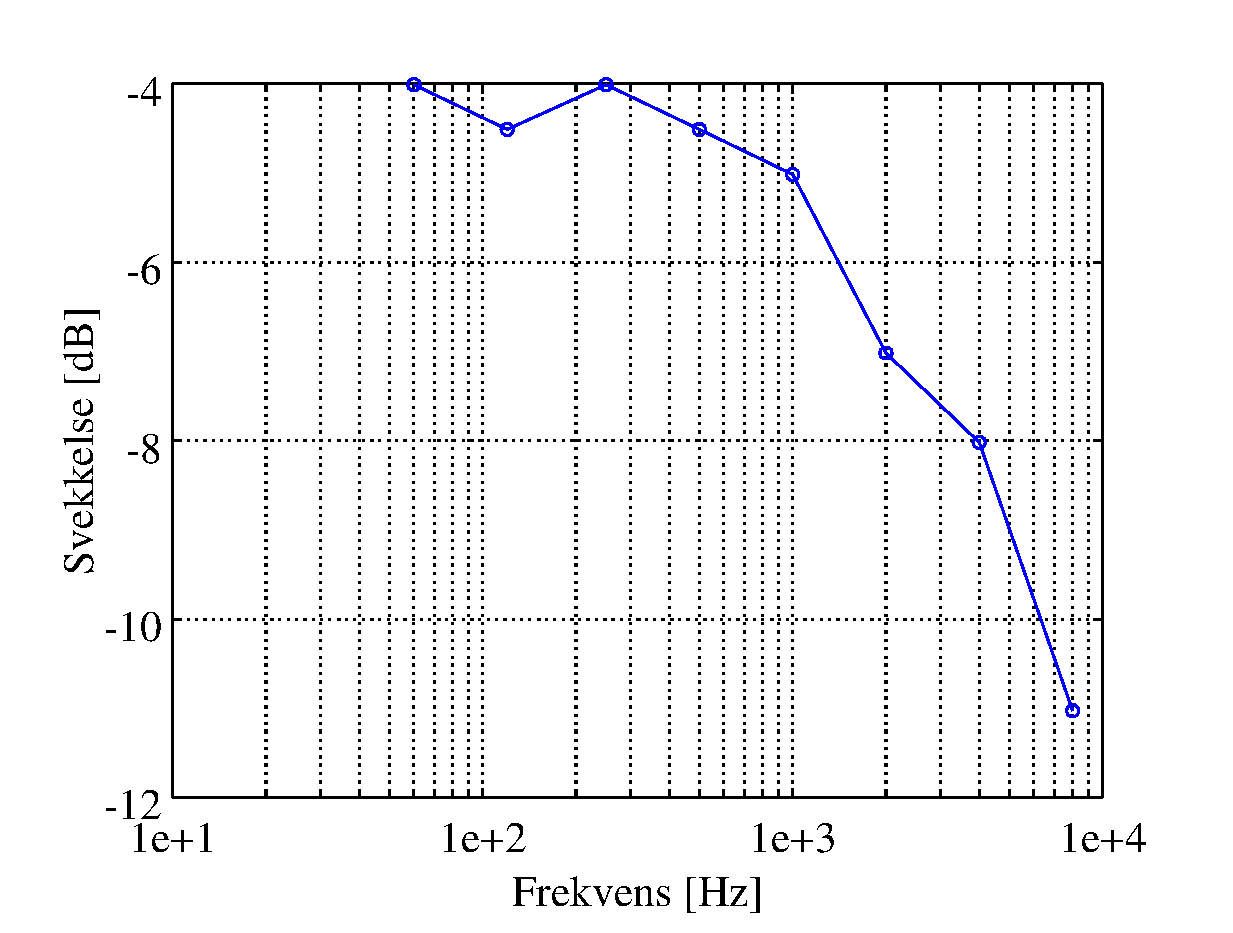
\includegraphics[width=100mm]{rightear35.eps}
	\caption[]{Audiogram for 35 år gammel mann. Høyre øre.}
	\label{fig:8}
\end{figure}
\begin{figure}[h!]
	\centering
	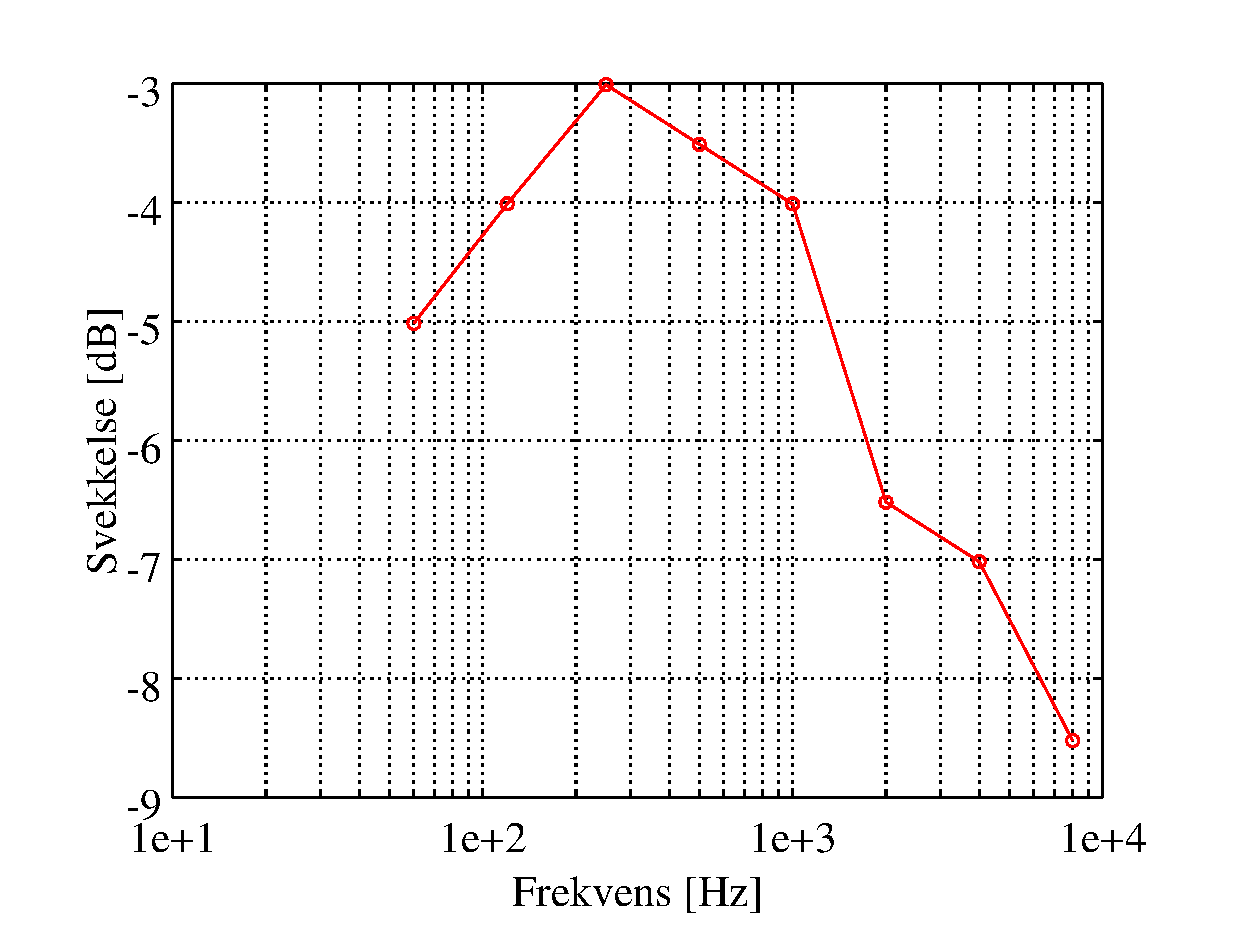
\includegraphics[width=100mm]{leftear35.eps}
	\caption[]{Audiogram for 35 år gammel mann. Venstre øre.}
	\label{fig:9}
\end{figure}
\begin{figure}[h!]
	\centering
	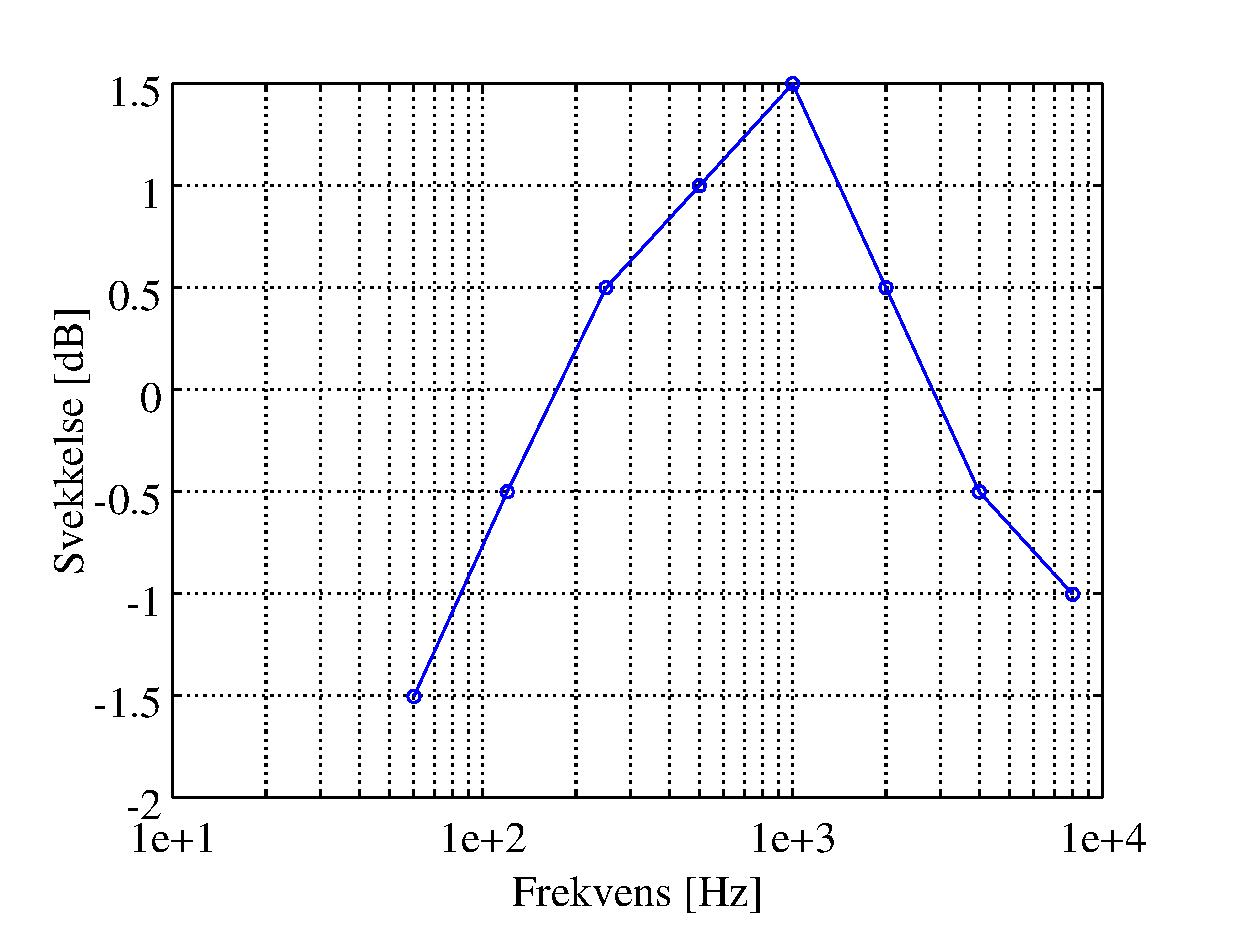
\includegraphics[width=100mm]{rightear18.eps}
	\caption[]{Audiogram for 18 år gammel kvinne. Høyre øre.}
	\label{fig:10}
\end{figure}
\begin{figure}[h!]
	\centering
	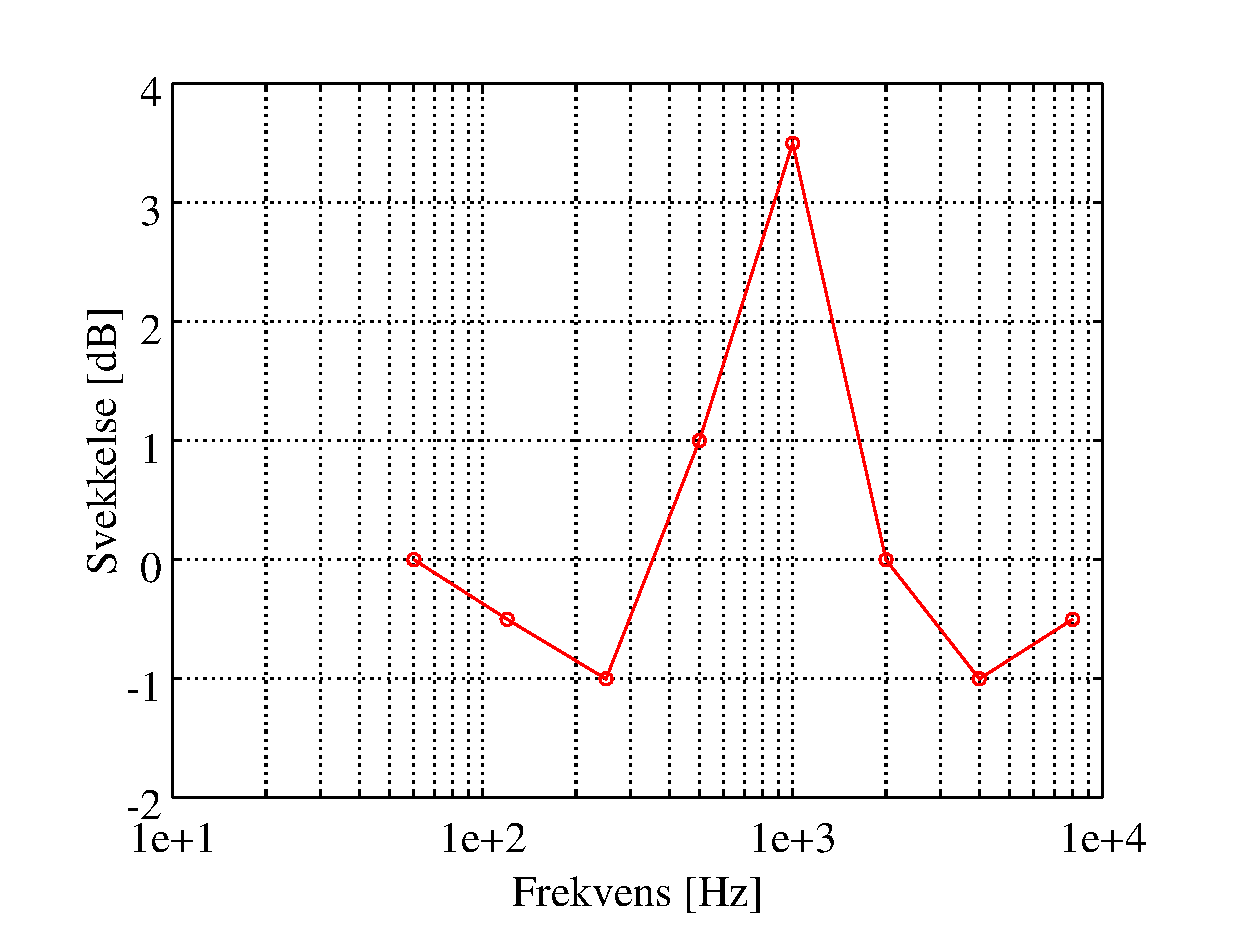
\includegraphics[width=100mm]{leftear18.eps}
	\caption[]{Audiogram for 18 år gammel kvinne. Venstre øre.}
	\label{fig:11}
\end{figure}
\end{document}